\subsection{Theory}
The K-Nearest Neighbour (K-NN) method is in this report used to classify a unknown digit to a set of known digits ranging from zero to nine.
%The data is split into two groups: One is for training and one is for testing. 
A set of the $k$ nearest neighbour is found using the euclidean distance to the pixel values in a training set with known values.
The result from the classification is found by counting the number of occurrences from the 
letting the $k$ voting between the K closest neighbours.

To see how this method performs a multitude of tests are performed to see how multiple parameters affect the success rate and the speed.


\begin{figure}[H]
\centering
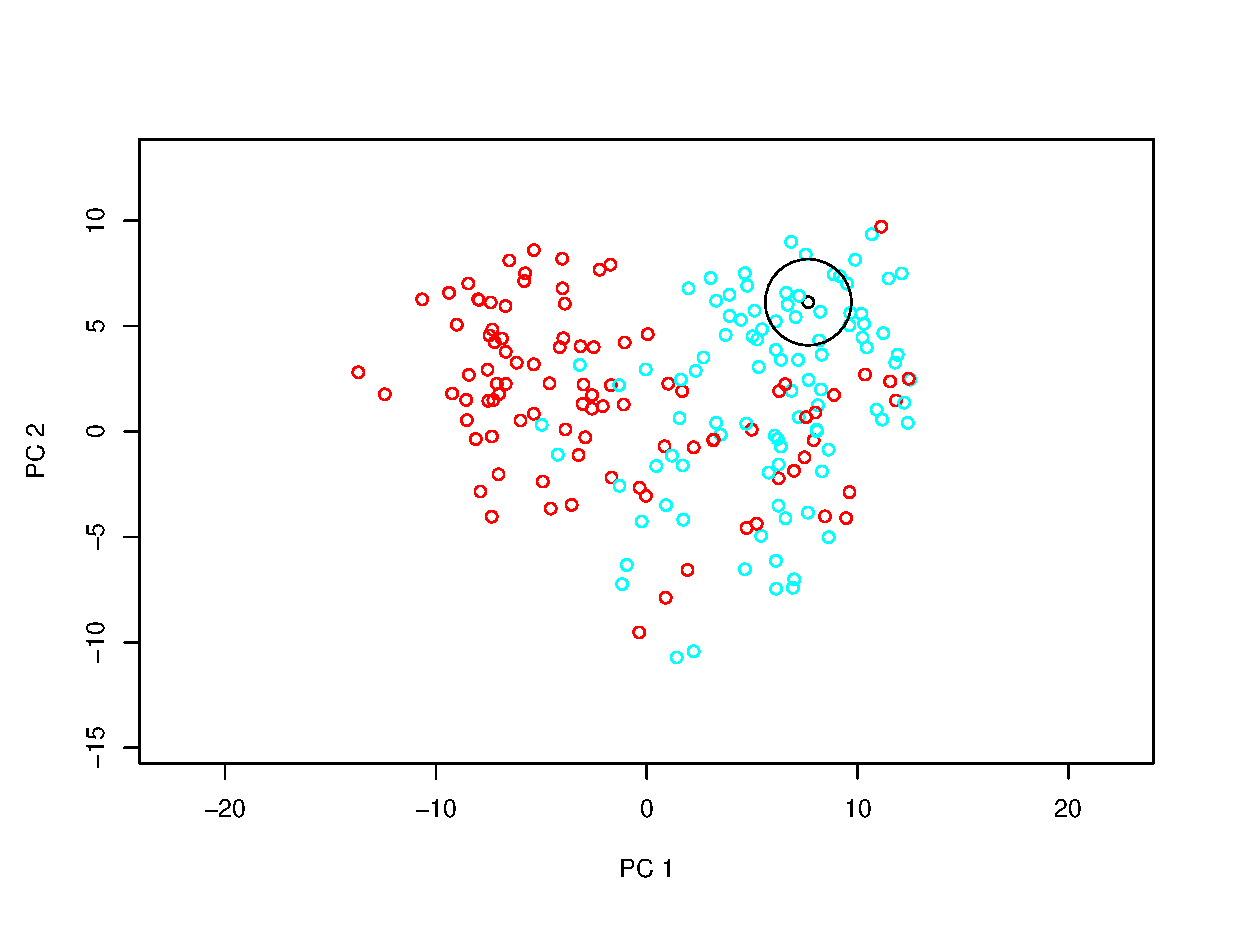
\includegraphics[width = 0.8 \textwidth]{graphics/knn_vis}
\caption{Illustration of the K-NN approach with $k = 10$.}
\label{fig:knn_illustration}
\end{figure}